\documentclass[12pt]{article}
% \usepackage[top=1in,left=1in, right = 1in, footskip=1in]{geometry}
\usepackage[top=1in,footskip=1in]{geometry}

\usepackage{graphicx}
\usepackage{xspace}
%\usepackage{adjustbox}

\usepackage{pdflscape}

\usepackage{grffile}

\newcommand{\comment}{\showcomment}
%% \newcommand{\comment}{\nocomment}

\newcommand{\showcomment}[3]{\textcolor{#1}{\textbf{[#2: }\textsl{#3}\textbf{]}}}
\newcommand{\nocomment}[3]{}

\newcommand{\jd}[1]{\comment{cyan}{JD}{#1}}
\newcommand{\swp}[1]{\comment{magenta}{SWP}{#1}}
\newcommand{\bmb}[1]{\comment{blue}{BMB}{#1}}
\newcommand{\djde}[1]{\comment{red}{DJDE}{#1}}

\newcommand{\eref}[1]{Eq.~(\ref{eq:#1})}
\newcommand{\fref}[1]{Fig.~\ref{fig:#1}}
\newcommand{\Fref}[1]{Fig.~\ref{fig:#1}}
\newcommand{\sref}[1]{Sec.~\ref{#1}}
\newcommand{\frange}[2]{Fig.~\ref{fig:#1}--\ref{fig:#2}}
\newcommand{\tref}[1]{Table~\ref{tab:#1}}
\newcommand{\tlab}[1]{\label{tab:#1}}
\newcommand{\seminar}{SE\mbox{$^m$}I\mbox{$^n$}R}

\usepackage{amsthm}
\usepackage{amsmath}
\usepackage{amssymb}
\usepackage{amsfonts}
\usepackage[utf8]{inputenc} % make sure fancy dashes etc. don't get dropped

\usepackage{lineno}
\linenumbers

\usepackage[pdfencoding=auto, psdextra]{hyperref}

\usepackage{natbib}
\bibliographystyle{chicago}
\date{\today}

\usepackage{xspace}
\newcommand*{\ie}{i.e.\@\xspace}

\usepackage{color}

\newcommand{\Rx}[1]{\ensuremath{{\mathcal R}_{#1}}\xspace} 
\newcommand{\RR}{\ensuremath{{\mathcal R}}\xspace}
\newcommand{\Rres}{\Rx{\mathrm{res}}}
\newcommand{\Rinv}{\Rx{\mathrm{inv}}}
\newcommand{\Rhat}{\ensuremath{{\hat\RR}}}
\newcommand{\Rt}{\ensuremath{{\mathcal R}(t)}\xspace}
\newcommand{\tsub}[2]{#1_{{\textrm{\tiny #2}}}}
\newcommand{\dd}[1]{\ensuremath{\, \mathrm{d}#1}}
\newcommand{\dtau}{\dd{\tau}}
\newcommand{\dx}{\dd{x}}
\newcommand{\dsigma}{\dd{\sigma}}

\newcommand{\rx}[1]{\ensuremath{{r}_{#1}}\xspace} 
\newcommand{\rres}{\rx{\mathrm{res}}}
\newcommand{\rinv}{\rx{\mathrm{inv}}}

\newcommand{\psymp}{\ensuremath{p}} %% primary symptom time
\newcommand{\ssymp}{\ensuremath{s}} %% secondary symptom time
\newcommand{\pinf}{\ensuremath{\alpha_1}} %% primary infection time
\newcommand{\sinf}{\ensuremath{\alpha_2}} %% secondary infection time

\newcommand{\psize}{{\mathcal P}} %% primary cohort size
\newcommand{\ssize}{{\mathcal S}} %% secondary cohort size

\newcommand{\gtime}{\tau_{\rm g}} %% generation interval
\newcommand{\gdist}{g} %% generation-interval distribution
\newcommand{\idist}{\ell} %% incubation-period distribution

\newcommand{\total}{{\mathcal T}} %% total number of serial intervals

\usepackage{lettrine}

\newcommand{\dropcapfont}{\fontfamily{lmss}\bfseries\fontsize{26pt}{28pt}\selectfont}
\newcommand{\dropcap}[1]{\lettrine[lines=2,lraise=0.05,findent=0.1em, nindent=0em]{{\dropcapfont{#1}}}{}}

\begin{document}

\begin{flushleft}{
	\Large
	\textbf\newline{
	  Interplay between climate-driven transmission and population-level susceptibility explains a sudden shift in RSV seasonality in Japan
	}
}
\newline
\\
Sang Woo Park, Inga, Emily, Wenchang, Gabe, Rachel Baker, Sarah Cobey, C. Jessica E. Metcalf, Bryan T. Grenfell
\bigskip
\end{flushleft}

\section*{Abstract} \swp{200 words. If we try for Nature Eco \& Evo, it needs to be $\leq 200$.}

Both endogenous and exogenous factors shape population-level ecological dynamics. Titrating their relative importance for dynamical transitions in host-pathogen systems remains a research frontier. Resolving this is an important step towards predicting future outbreaks and making public health decisions.
In Japan, respiratory syncytial virus (RSV), a major childhood respiratory pathogen, displayed a sudden, dramatic shift in outbreak seasonality (from winter to fall) in 2016. We use mathematical models to identify processes that could lead to this outcome.
In line with previous analyses, we identify a robust quadratic relationship between mean specific humidity and transmission, with minimum transmission occurring at intermediate humidity.
This drives semiannual patterns of seasonal transmission rates that peak in summer and winter.
Under this transmission regime, we find that a subtle increase in population-level susceptibility can cause a sudden shift in seasonality, where the degree of shift is primarily determined by the lag between the two peaks of seasonal transmission rate.
We hypothesize that an increase in children attending childcare facilities following the launch of the Comprehensive Support System for Children and Childcare in Japan may have contributed to the increase in susceptibility through increased contact rates.
Our analysis underscores the power of studying infectious disease dynamics to titrate the roles of underlying drivers of dynamical transitions in ecology.

\pagebreak

\section*{Introduction}

Characterizing the drivers of dynamical transitions is a fundamental challenge in ecology \citep{earn2000simple,hastings2004transients,hastings2018transient}.
However, time series data from ecological systems are rare, and, where they do exist, sparse; reducing our ability to tease apart the relative roles of endogenous (e.g., density-dependent responses) and exogenous (e.g., climate variables) factors in driving dynamical transitions \citep{hunter1998cycles,lundberg2000population,hernandez2012fluctuations}.
There is one important exception: detailed spatiotemporal surveillance data are available for many epidemiological systems, providing a unique platform for answering broader questions in ecology and population biology \citep{levin1997mathematical,anderson1991infectious,grenfell2001travelling,he2010plug}.

Respiratory syncytial virus (RSV) is a common childhood respiratory pathogen that infects nearly all children by the age of two, and is also an important risk factor for asthma and allergy development \citep{sigurs1995asthma,sigurs2010asthma,edwards2012microbiology}.
RSV outbreaks typically exhibit annual or biennial patterns with relatively consistent seasonal incidence across years in many countries, including Canada \citep{paramo2023respiratory}, Korea \citep{kim2020investigation}, and the US \citep{pitzer2015environmental,baker2019epidemic}.
Previous studies showed that climate-driven transmission plays a major role in driving RSV epidemic dynamics \citep{pitzer2015environmental,baker2019epidemic}.
In particular, \cite{baker2019epidemic} demonstrated a quadratic relationship between specific humidity and RSV transmission with minimum transmission occurring at intermediate humidity.

RSV in Japan presents a unique case study relative to other countries: In contrast to stable seasonal incidence generally observed, a sudden, dramatic transition from winter to fall RSV outbreaks was observed in Japan in 2016 \citep{miyama2021seasonal,wagatsuma2021shifts}.
\cite{wagatsuma2021shifts} hypothesized that changes in climate and an increase in inbound overseas travelers may be jointly responsible for this shift in seasonality.
However, their conclusion relied on correlational analyses, and little ecological support was provided for their proposed mechanism.
Understanding the sudden shift in RSV seasonality is a necessary step for predicting future RSV outbreaks, as well as for timely deployment of monoclonal antibodies and vaccination \citep{mazur2023respiratory}.

Here, we analyzed the time series of RSV cases from Japan (\fref{fig1}) to identify the drivers of a sudden shift in seasonality between 2016 and 2017. 
We combined a parsimonious model of disease transmission with Bayesian statistical framework to infer RSV transmission patterns across different islands.
We used inferred transmission patterns to explore how changes in susceptibility can lead to a sudden shift in seasonality.
Our analysis offers novel insights into drivers of dynamical transition in seasonal respiratory epidemics.

\section*{Results}

\subsection*{Observed dynamics in RSV outbreaks}

\begin{figure}[!th]
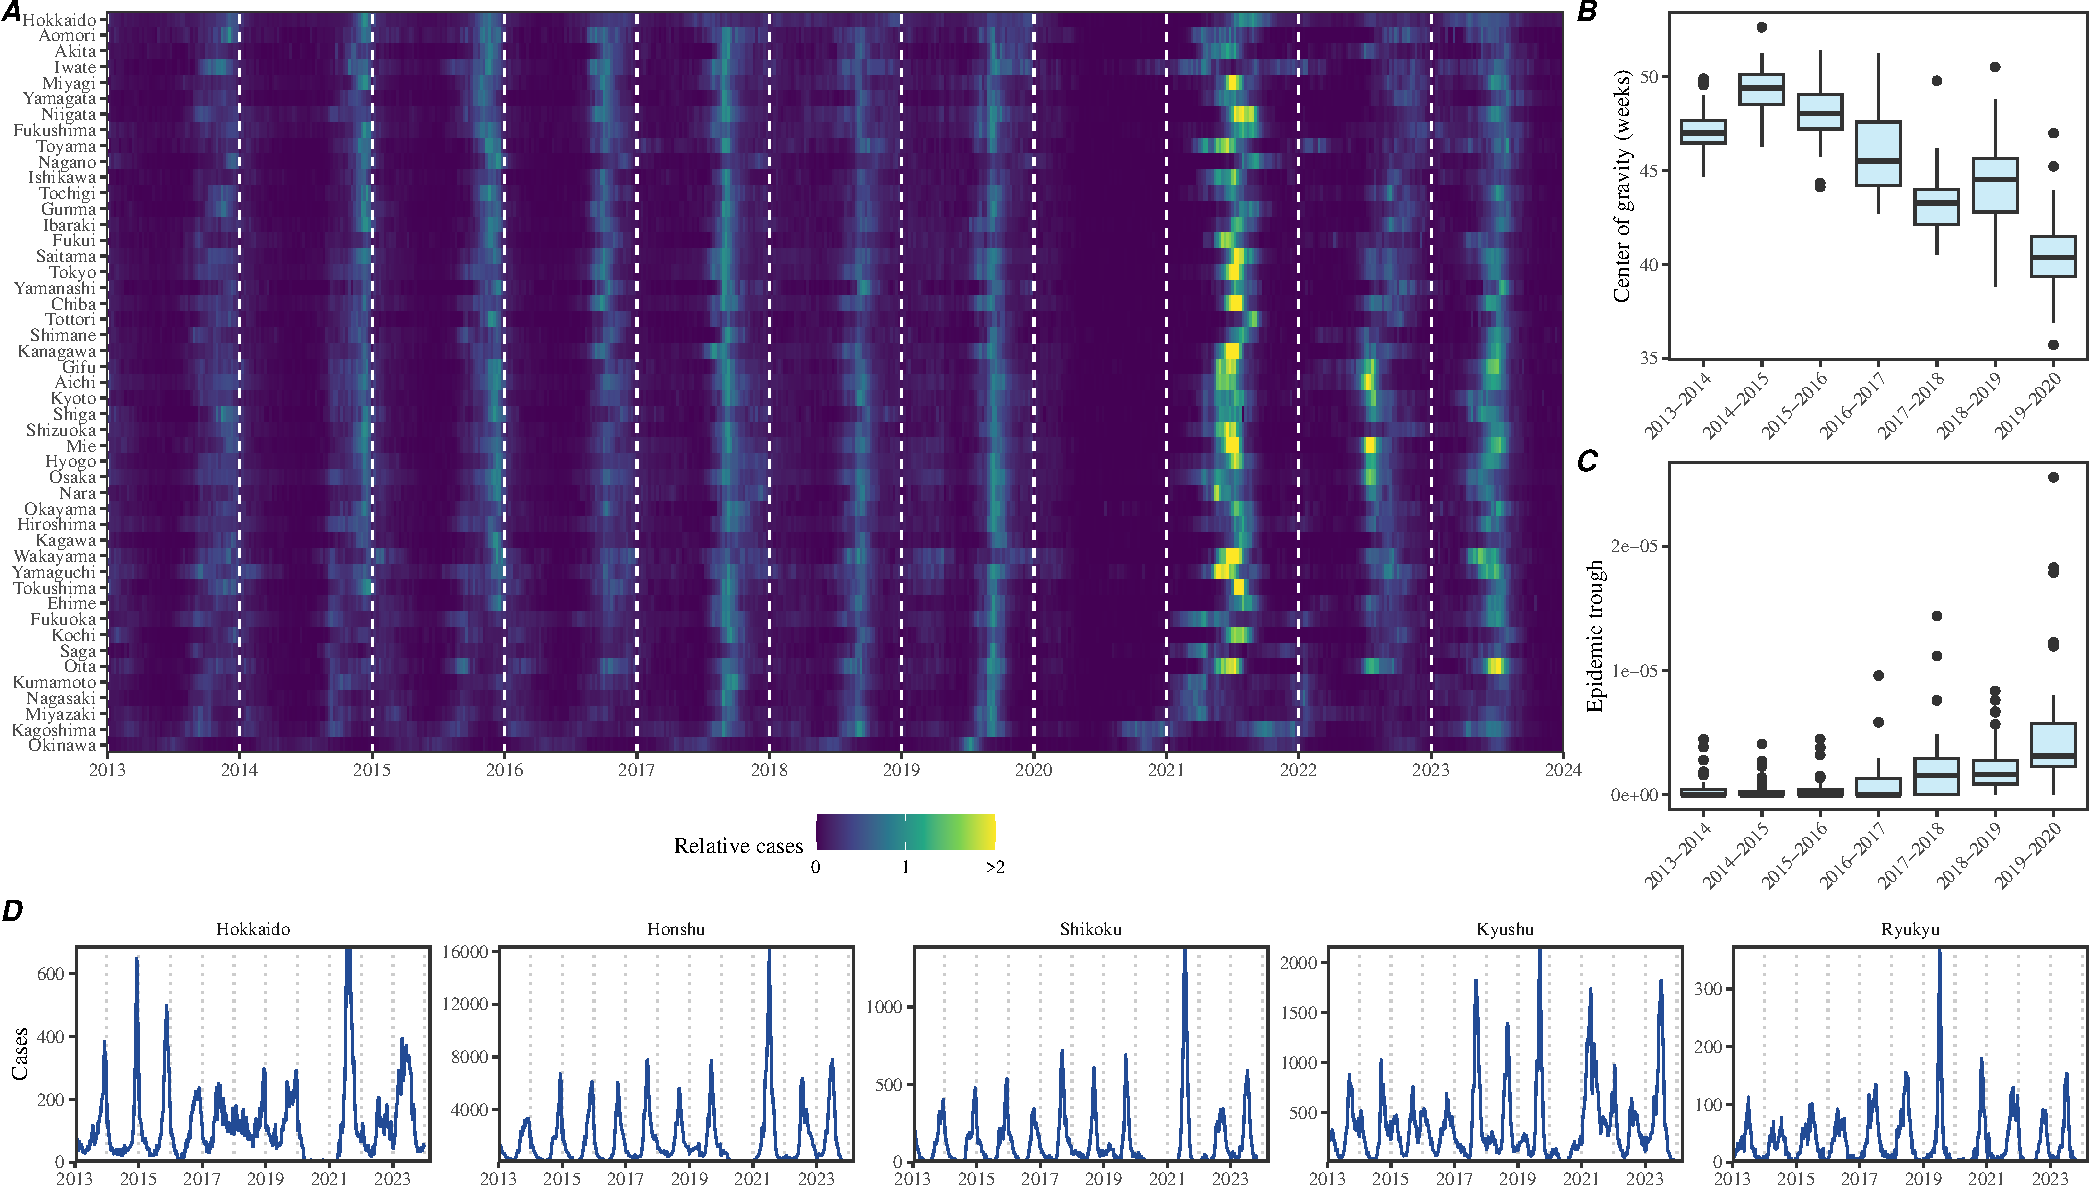
\includegraphics[width=\textwidth]{../figure/figure1.pdf}
\caption{
\textbf{Observed changes in RSV outbreak dynamics in Japan.}
(A) Relative RSV cases across 47 prefectures in Japan between 2013 and 2024.
Relative cases are calculated by dividing the raw cases by the pre-pandemic maximum.
The red arrow indicates when the shift in seasonality occurred.
(B) Estimates of center of gravity (i.e., the mean timing of an epidemic) across 46 prefectures, excluding Okinawa.
(C) Estimates of the epidemic trough (i.e., the minimum number of cases in a season divided by the population size) across 47 prefectures.
(D) Time series of RSV cases across 5 major islands.
}
\label{fig:fig1}
\end{figure}

A sudden change in RSV seasonality from winter to fall outbreaks was observed in nearly all prefectures between 2016 and 2017 (\fref{fig1}A).
To quantify changes in seasonality, we calculated the center of gravity (i.e., the mean timing of an epidemic) for each outbreak season at every prefecture and found a consistent decrease in the center of gravity (\fref{fig1}B; Methods). 
We also found that these changes were associated with the inter-epidemic troughs becoming shallower (\fref{fig1}C).

We found considerable heterogeneity in the observed outbreak dynamics across the major islands, especially following the changes in seasonality (\fref{fig1}D).
For example, annual RSV outbreaks in Hokkaido island became more persistent, causing high numbers of cases throughout the year.
Semiannual RSV outbreaks in Shikoku and Kyushu islands became more annual with higher intensity, leading to sharper epidemics.
Finally, in contrast to all other islands, RSV outbreaks in Ryukyu island exhibited summer outbreaks, which also became more intense leading up to 2020.

\subsection*{A parsimonious model for RSV epidemics}

We first began by asking whether a simple Susceptible-Infected-Recovered-Susceptible (SIRS) model can capture the observed RSV outbreak dynamics in Japan, including the sudden change in outbreak seasonality.
The SIRS model is the simplest model that allows for the possibility of immune waning and therefore represents one of the most parsimonious models for explaining outbreak dynamics of respiratory infections.
Here, we extended the standard SIRS model such that we could simultaneously estimate periodic seasonal transmission rates and non-periodic changes in transmission due to NPI measures that were implemented to prevent COVID-19  (Methods).

\begin{figure}[!th]
\includegraphics[width=\textwidth]{../figure/figure_comb_sirs_npi.pdf}
\caption{
\textbf{Summary of SIRS model fits to RSV outbreaks across major islands in Japan.}
(A) Comparisons of observed cases (points) across the five major islands and fitted epidemic trajectories (red lines).
(B) Estimated periodic seasonal transmission rates.
(C) Relationship between the estimated periodic seasonal transmission rates and mean specific humidity.
Points represent seasonal transmission rate estimates across 52 weeks versus average humidity across 2013--2020.
Lines represent the corresponding locally estimated scatterplot smoothing (LOESS) estimates.
(D) Estimated relative changes in transmission, capturing the impact of NPI measures.
(E) Estimated proportion of the susceptible pool.
Lines represent the estimated median of the posterior distribution.
Shaded regions represent the 95\% credible intervals from the posterior distribution.
}
\label{fig:fig2}
\end{figure}

The SIRS model was able to reproduce the observed dynamics across all five islands, including changes in seasonality that occurred during 2016--2017 as well as post-pandemic changes in outbreak patterns (\fref{fig2}A).
Interestingly, we estimated semiannual peaks in transmission rates across all islands, except for Hokkaido (\fref{fig2}B).
These semiannual patterns in transmission were explained by the nonlinear effects of specific humidity:
in line with \cite{baker2019epidemic}, we estimated that transmission would peak at a low and high mean specific humidity (\fref{fig2}C).
Interestingly, we found that this quadratic relationship between mean specific humidity and transmission rates was robust across four islands (Honshu, Shikoku, Kyushu, and Ryukyu), with Ryukyu island exhibiting minimum RSV transmission at a much higher mean specific humidity than other islands (\fref{fig2}C).
Combining transmission rate estimates from all five islands still yield a quadratic relationship but the joint relationship poorly capture the humidity-transmission relationship in the Ryukyu island (Supplementary Figure S1).

Across all five islands, we estimated a considerable reduction in transmission during 2020  (\fref{fig2}D);
however, there was large heterogeneity in the overall shape of the estimated NPI effects as well as the degree of transmission reduction.
The reduction in transmission rates caused an increase in the susceptible pool (\fref{fig2}E), which allowed a large outbreak when NPIs were lifted (\fref{fig2}A);
this is also consistent with \cite{baker2019epidemic}.

\subsection*{Mechanisms for sudden changes in seasonality}

Since our SIRS model could accurately capture the observed dynamics, we were able to use our fits to further tease apart the mechanisms underlying sudden changes in seasonality of the RSV outbreaks.
To do so, we first began by evaluating the changes in the proportion of susceptible and infected individuals at the beginning of the season between 2013 and 2019;
we focused on three main islands that exhibited clear changes in seasonality: Honshu, Shikoku, and Kyushu islands. 

We found a consistent increase in the proportion of susceptible and infected individuals at the beginning of each season between 2013 and 2019 across three main islands (\fref{fig3}A).
These changes also corresponded with a decrease in center of gravity (\fref{fig3}A).
A more detailed comparison of epidemic trajectories illustrated that an increase in the susceptible pool at the beginning of the season can drive a sudden shift in seasonality (\fref{fig3}B).

We also found considerable heterogeneity across islands in differences in peak epidemic timing associated with changes in seasonality (\fref{fig3}B): 9--12 weeks (Honshu), 6--11 weeks (Shikoku), and 18--20 weeks (Kyushu).
This heterogeneity can be explained by the differences in the seasonal transmission patterns (\fref{fig3}C--G).
Specifically, RSV transmission in Honshu island (\fref{fig3}C) exhibits a narrower amplitude (\fref{fig3}D) and a narrower trough (\fref{fig3}E) compared to RSV transmission in Honshu island (\fref{fig3}E).
Simulating the SIRS model using seasonal transmission rates that interpolate those estimated from two islands confirmed that a large seasonal amplitude and wider trough cause larger changes in the timing of epidemic peak (\fref{fig3}F). 

\begin{figure}[!th]
\includegraphics[width=\textwidth]{../figure/figure_comb_sirs_change.pdf}
\caption{
\textbf{An increase in the susceptible pool explains sudden changes in seasonality.}
(A) Predicted effects of the proportion of infected $i(0)$ and susceptible $S(0)$ at the beginning of season on center of gravity.
Points represent the estimated values for $i(0)$ and $s(0)$ between 2013 and 2019.
(B) Changes in epidemic trajectories caused by an increase in the susceptible proportion at the beginning of season for a fixed value of $i(0)$ (white dashed line in panel A).
(C--F) Comparisons of interpolated transmission rates used for simulating the SIRS model, corresponding to each corner in Panel G. 
Black lines represent the transmission rates used for simulations. 
Gray lines represent the estimated transmission rates the Honshu island as a visual reference.
(C) The estimated transmission rates for the Honshu island.
(D) The resulting transmission rates for the Honshu island when we increase the amplitude to match the amplitude of the transmission rates for the Kyushu island.
(E) The resulting transmission rates for the Kyushu island when we decrease the amplitude to match the amplitude of the transmission rates for the Honshu island.
(F) The estimated transmission rates for the Kyushu island.
(G) Differences in peak epidemic timing when we increase the the susceptible proportion at the beginning of season from 7.8\% to 10.5\% across different assumptions about the underlying transmission rate. 
}
\label{fig:fig3}
\end{figure}

\subsection*{Mechanisms for an increase in population-level susceptibility}

So what mechanisms caused the population-level susceptibility to increase over time in Japan?
We hypothesized that the Comprehensive Support System for Children and Childcare, which was enacted in 2012 and launched in 2015, contributed to an increase in population-level susceptibility.
An expansion of childcare facilities would increase contact rates among children, which in turn would increase the probability of exposure and therefore the effective susceptibility against RSV infections.
To quantify the potential impact of this program, we compared the number of children attending childcare facilities in Japan since 2013 and compared them with our estimates of susceptible proportion (\fref{fig4}).
Overall, we found consistent patterns of increase in childcare attendance and strong correlations with the estimated susceptible proportion: 0.977 (95\% CI: 0.847--0.997) in Honshu island, 0.943 (95\% CI: 0.653--0.992) in Shikoku island, and 0.802 (95\% CI: 0.124--0.970) in Kyushu island.

\begin{figure}[!th]
\includegraphics[width=\textwidth]{../figure/figure_childcare.pdf}
\caption{
\textbf{Increase in the susceptible pool following the launch of the Comprehensive Support System for Children and Childcare in Japan.}
(A) Direct comparisons between the estimates of susceptible proportion at the beginning of each season in each island (black) and the number of children attending childcare facilities in Japan (red).
Shaded regions represent the 95\% credible interval in our estimates.
(B) Correlations between the estimates of susceptible proportion at the beginning of each season in each island and the number of children attending childcare facilities in Japan.
Error bars represent  the 95\% credible interval in our estimates.
Red lines and shaded regions represent the best fitting linear regression and the corresponding 95\% confidence intervals.
}
\label{fig:fig4}
\end{figure}

\section*{Discussion}

We present an epidemiological analysis of RSV outbreaks in Japan using mathematical modeling approach.
Our analysis revealed semiannual cycles in seasonal RSV transmission, which correlate with specific humidity.
We found that these semiannual cycles allowed a sudden shift in the seasonality of RSV outbreaks through an increase in population-level susceptibility.
We  hypothesize that an increase in childcare capacity in Japan may be a main driver of the increase in population-level susceptibility.

Our analysis revealed considerable heterogeneity in epidemic dynamics across major islands in Japan.
We showed that these differences could be explained by the differences in underlying seasonal transmission.
Notably, we found a robust, quadratic relationship between the estimated transmission rates and mean specific humidity across four major islands (Honshu, Shikoku, Kyushu, and Ryukyu), indicating low transmission at intermediate levels of specific humidity.
These findings echo earlier studies that demonstrated similar relationships for RSV \citep{baker2019epidemic} and influenza \citep{tamerius2013environmental}.
The robustness of this quadratic relationship across islands exhibiting different climate conditions suggests a possibility that climate-driven transmission may be, in part, facilitated by human behavior: for example, an increase in time spent indoors during low and high humidity seasons can contribute to increased transmission.
We note that this relationship is correlational, rather than causal, and therefore any other climate variables (e.g., temperature) or seasonal variation in human behavior (e.g., school terms) that correlate with seasonal variation in specific humidity will be implicitly captured by this relationship.

We tentatively hypothesized that the Comprehensive Support System for Children and Childcare may have contributed to the increase in population-level susceptibility, but other mechanisms may have contributed as well.
For example, \cite{wagatsuma2021shifts} hypothesized that changes in climate and an increase in inbound overseas travelers may be both responsible for this shift in seasonality.
While an increase in overseas travelers may also contribute to the increase in contact rates and therefore the effective susceptibility against RSV, it is likely to have weak effects given that the mean age of infection for RSV is typically very young.
Our findings are consistent with those by \cite{dehaan2024age} who also suggested that an increase in childcare attendance may have contributed to a large change in the seasonality of Kawasaki disease in Japan in the mid-2010s.

Interventions to slow the transmission of COVID-19 have disrupted the circulation of many pathogens \citep{baker2020impact,eden2022off,chen2024covid,park2024predicting}, including RSV epidemics in Japan.
This disruption has added major challenges to predicting future outbreaks, which prevented us from making long-term predictions.
Continued analysis of RSV dynamics in the post-COVID period, particularly with regard to whether RSV outbreaks in Japan return to fall or winter outbreaks, may help further validate our models.

Our analysis relied on several simplifying assumptions.
For example, our model assumed complete waning of immunity.
In practice, immunity is likely more complex with secondary infections being less susceptible and transmissible than primary infections \citep{pitzer2015environmental}.
Other studies have also suggested the importance of interaction between RSV A and B \citep{white2005transmission,holmdahl2024differential} as well as competition between RSV and human metapneumovirus \citep{bhattacharyya2015cross}; 
our model did not account for such strain dynamics.
We also did not account for explicit spatial structure or underlying stochasticity of the system.
Despite these limitations, our model likely represents a parsimonious approximation of the complex host-pathogen interactions, allowing us to draw general conclusions about how interactions between endogenous (population-level susceptibility) and exogenous (climate-driven factors) factors can give rise to a sudden dynamical transition.

Understanding how endogenous and exogenous factors shape epidemic dynamics is critical to predicting future outbreaks and making public health decisions.
Our analysis shows that the interplay between climate-driven transmission and subtle changes in population-level susceptibility can cause a sudden transition in epidemic dynamics.
More broadly, our analysis demonstrates that detailed epidemiological time series data can allow us to tease apart endogenous and exogenous factors in explaining dynamical transitions, offering unique insights into a long-standing ecological question.

\section*{Materials and methods}

\subsection*{Epidemiological data}

The Japan prefecture-level weekly time series of RSV cases comes from the National Institute of Infectious Diseases (NIID).
The NIID issues Infectious Diseases Weekly Report (IDWR) every week, which includes sentinel-reporting diseases.
We downloaded all available IDWR surveillance tables for sentinel-reporting diseases from the beginning of 2013 to end of 2023 from \url{https://www.niid.go.jp/niid/en/survaillance-data-table-english.html} and extracted RSV time series from these tables.

\subsection*{Demographic data}

Population sizes for each prefecture as of 2022 were obtained from Statistics of Japan website (\url{https://www.e-stat.go.jp/en}).
Statistics on the number of children attending childcare facilities were obtained from the Children and Families Agency website (\url{cfa.jp.gov}).

\subsection*{Climate data}

The specific humidity data used in this study is from European Centre for Medium-Range Weather Forecasts (ECMWF) Reanalysis v5 (ERA5) \citep{hersbach2020era5}. 
The original data are houly with a horizontal resolution of about 31km. 
We first resample the hourly data to obtain daily mean values and then perform spatial average over cell grids within each prefecture in Japan. 
We further summarized the daily time series of specific humidity into weekly mean values in each prefecture, which were further averaged over to obtain weekly mean values in each island.

\subsection*{Center of gravity and epidemic trough}

In order to characterize changes in the timing of the epidemic, we quantified the center of gravity of RSV cases for each RSV season at each prefecture.
Here, we excluded the Okinawa prefecture, which the southernmost prefecture of Japan, due to differences in RSV seasonality:
in contrast to all other prefectures that exhibit winter outbreaks, summer outbreaks are observed in the Okinawa prefecture.
To compute the center of gravity, we defined the RSV season from week 27 of the current year to week 26 of the next year and numbered each week of season from 1 (starting from week 27 of a given year) to 52 (ending at week 26 of the following year).
Then, for each season, we calculated center of gravity by taking the weighted mean of the week of season, weighted by the number of cases.
We added 26 to the resulting center of gravity to convert the estimates to be in the units of regular weeks (rather than the week of season).
For each season, we also quantified the corresponding epidemic trough by taking the minimum value of weekly cases.
For the 2019--2020 season, we took the minimum cases before 2020 to exclude the impact of COVID-19 interventions.

\subsection*{Transmission and observation model}

To model the population-level spread of RSV in Japan, we extended the standard Susceptible-Infected-Recovered-Susceptible (SIRS) model to account for non-sinusoidal seasonal transmission rates and changes in transmission patterns due to COVID-19 intervention measures.
Specifically, the discrete-time SIRS model is given by:
\begin{align}
\mathrm{FOI}(t) &= \frac{\beta(t) (I(t) + \omega)}{N}\\
\Delta S(t) &= \left[1- \exp(-(\mathrm{FOI}(t) + \mu) \Delta t )\right] S(t-\Delta t)\\
N_{SI}(t) &= \frac{\mathrm{FOI}(t)\Delta S(t)}{\mathrm{FOI}(t) + \mu} \\
\Delta I(t) &= \left[1- \exp(-(\gamma + \mu) \Delta t )\right] I(t-\Delta t)\\
N_{IR}(t) &= \frac{\gamma \Delta I(t)}{\gamma + \mu} \\
\Delta R(t) &= \left[1- \exp(-(\nu + \mu) \Delta t )\right] R(t-\Delta t)\\
N_{RS}(t) &= \frac{\nu \Delta R(t)}{\nu + \mu} \\
S(t) &= S(t-\Delta t) + \mu N - \Delta S(t) + N_{RS}(t)  \\
I(t) &= I(t-\Delta t) - \Delta I(t) + N_{SI}(t)  \\
R(t) &= R(t-\Delta t) - \Delta R(t) + N_{IR}(t)  \\
\end{align}
Here, $S$, $I$, and $R$ represent the number of individuals who are susceptible, infected, and recovered;
$N$ represents the total population size;
$\mathrm{FOI}(t)$ represents the force of infection at time $t$;
$\Delta X(t)$ represents number of individuals who leave the compartment $X$ at time $t$;
$N_{XY}(t)$ represents the number of individuals who move from compartment $X$ to compartment $Y$ at time $t$;
$\beta(t)$ represents the time-varying transmission rate;
$\omega$ represents the number of imported infections;
$\gamma$ represents the recovery rate;
$\nu$ represents the immune waning rate;
and $\mu$ represents the birth and death rates.

Typically, the transmission rate is assumed to follow a sinusoidal function for modeling endemic diseases.
Instead, we decomposed $\beta(t)$ into a product of two separate terms:
\begin{equation}
\beta(t) = \tsub{\beta}{seas}(t) \delta(t),
\end{equation}
where $\tsub{\beta}{seas}(t)$ represents the seasonal transmission rate and $\delta(t)$ represents relative changes in transmission due to COVID-19 intervention measures, such that $\delta < 1$ represents transmission reduction.
A similar decomposition was recently used for modeling the spread of Mycoplasma pneumoniae infections \citep{park2024myco}.

First, we modeled the seasonal transmission rate $\tsub{\beta}{seas}(t)$ as a periodic function with a period of 52 weeks ($\tsub{\beta}{seas}(t) = \tsub{\beta}{seas}(t-52)$) and tried to estimate a separate value for each week.
To constrain the shape of $\tsub{\beta}{seas}(t)$, we imposed cyclic random-walk priors:
\begin{align}
\tsub{\beta}{seas}(t+1) &\sim \mathrm{Normal}(\tsub{\beta}{seas}(t), \tsub{\sigma}{seas}), \quad t=1,\dots,51  \\
\tsub{\beta}{seas}(1) &\sim \mathrm{Normal}(\tsub{\beta}{seas}(52), \tsub{\sigma}{seas})
\end{align}
where the standard deviation $\tsub{\sigma}{seas}$ determines the smoothness of the seasonal transmission rate.
We imposed a weakly informative prior on $\tsub{\sigma}{seas}$:
\begin{equation}
\tsub{\sigma}{seas} \sim \textrm{Half-Normal}(0, 1).
\end{equation}
To further constrain the range of seasonal transmission rate $\tsub{\beta}{seas}(t)$, we imposed additional priors:
\begin{equation}
\tsub{\beta}{seas}(t) \sim \mathrm{Normal}(8, 2).
\end{equation}

Second, we assumed $\delta(t) = 1$ for $t < 2020$ (before the COVID-19 pandemic) and tried to estimate a separate value for $\delta(t)$ at each week.
To constrain the shape of $\delta(t)$, we imposed random-walk priors:
\begin{align}
\delta(t+1) &\sim \mathrm{Normal}(\delta(t), \sigma_\delta), \quad t \geq 2020
\end{align}
where the standard deviation $\tsub{\sigma}{seas}$ determines the smoothness of the estimated $\delta(t)$.
We imposed a weakly informative prior on $\sigma_\delta$:
\begin{equation}
\sigma_\delta \sim \textrm{Half-Normal}(0, 0.1).
\end{equation}
To further constrain the range of estimated intervention effects $\delta$, we imposed additional priors:
\begin{equation}
\delta(t) \sim \mathrm{Normal}(1, 0.2).
\end{equation}
For the analysis of Hokkaido island, we estimated $\delta(t)$ beginning from 2017 instead of 2020 to capture sudden changes in epidemic dynamics.

We assumed that the recovery rate $\gamma = 1/\mathrm{week}$ and birth/death rates $\mu = 1/(80\times 52)\,\mathrm{weeks}$ are known.
We imposed weakly informative priors on all other parameters:
\begin{align}
1/\nu &\sim \textrm{Half-Normal}(0, 200)\\
\omega &\sim \textrm{Half-Normal}(0, 200)\\
s(0) &\sim \textrm{Normal}(0.08, 0.02)\\
i(0) &\sim \textrm{Half-Normal}(0, 0.001)\\
\end{align}
where $s(0)$ and $i(0)$ represent the initial proportion of susceptible and infected individuals such that the initial conditions are given by: $S(0) = Ns(0)$ and $I(0) = N i(0)$.

Finally, the model was fitted to case data in each island by assuming a negative binomial observation error:
\begin{align}
C(t) &= N_{SI}(t)\\
\textrm{cases}_t &\sim \textrm{Negative-Binomial}(\rho C(t), \phi)\\
\rho &\sim \textrm{Half-Normal}(0, 0.02)\\
\phi &\sim \textrm{Half-Normal}(0, 10)
\end{align}
where $C(t)$ represents the incidence of infection, $\rho$ represents the under-reporting rate, and $\phi$ represents the overdispersion parameter.
Parameter estimation was performed in a Bayesian framework using the rstan package \citep{carpenter2017stan}.
Convergence was assess by ensuring low R-hat, high effective sample size, no divergent transitions, and no iterations that exceeded the maximum tree depth.
The model struggled to converge for the analysis of Shikoku island---in this case, removing the $\mathrm{Normal}(1, 0.2)$ prior on $\delta(t)$ allowed us to fit the model.

\subsection*{Simulations}

We run a series of simulations to understand how the interplay between climate-driven transmission and population-level susceptibility can drive a sudden shift in the timing of an epidemic.
First, we simulated the model for a year (from week 26 of the starting year to week 25 of the following year) by varying the initial conditions and computing the center of gravity.
Specifically, we varied $i(0)$ between $1\times 10^{-4}$ and $3\times 10^{-3}$ and $s(0)$ between $0.078$ and $0.105$.
All other parameters were set to posterior median estimates.

To further understand how the shape of seasonal transmission term affects the degree of shift in seasonality, we varied the shape of seasonal transmission term by interpolating the estimated $\tsub{\beta}{seas}$ from Honshu and Kyshu islands, which are the two most populated islands. 
To do so, we first took posterior median estimates of $\tsub{\beta}{seas}$ from two islands and fitted generalized additive model with cyclic cubic spline bases to obtain smoothed estimates of $\tsub{\beta}{seas}$ for each island, which we denote as $\beta_H$ and $\beta_K$, respectively.
Then, we normalized seasonal transmission rates such that it has a mean of zero and has an amplitude of 1:
\begin{equation}
\zeta_X(t) = \frac{1}{\alpha_X} \left(\frac{\beta_{X}(t)}{\bar{\beta}_X} - 1\right)
\end{equation}
where $\zeta_X(t)$ represents the normalized seasonal transmission pattern in island $X$,
and $\alpha_X = (\max(\beta_X(t)) - \min(\beta_X(t)))/2$ represents the amplitude of seasonal transmission pattern in island $X$.
This allowed us to interpolate between two normalized seasonal terms and obtain a flexible shape for seasonal transmission rate:
\begin{align}
\tsub{\zeta}{new}(t) &= \zeta_H(t) (1-\theta) + \zeta_K(t)(\theta),\\
\tsub{\beta}{new} &= \left(\frac{\tsub{\alpha}{new} \tsub{\zeta}{new}(t)}{(\max(\tsub{\zeta}{new}(t))-\min(\tsub{\zeta}{new}(t)))/2} + 1\right) \tsub{\bar{\beta}}{new},
\end{align}
where $\theta$ represents the interpolation coefficient, such that $\theta=0$ and $\theta=1$ causes $\tsub{\beta}{new}$ to have the same shape as $\beta_H$ and $\beta_K$, respectively and $0 < \beta < 1$ allows us to model counterfactual transmission scenarios that interpolates between two islands.
Note that $\tsub{\zeta}{new}(t)$ does not necessarily have an amplitude 1 so we divide it by $(\max(\tsub{\zeta}{new}(t))-\min(\tsub{\zeta}{new}(t)))/2$ to ensure the amplitude of 1.

For a given value of the interpolation coefficient $\theta$ and seasonal amplitude $\tsub{\alpha}{new}$, we simulated two outbreaks for a year assuming $s(0) = 0.078$ and $s(0)=0.105$ and computed the difference in the timing of epidemic peak.
In doing so, all other parameters, including the mean transmission rate $\tsub{\beta}{new}$, were fixed to posterior median estimates for the Honshu island. 

\subsection*{Regression}

We also performed a linear regression between the estimated proportion of susceptibles at the beginning of each season (week 26) against the number of children attending childcare facilities.
For simplicity, the regression was performed using median estimates for the susceptible proportions.
We did not have data on the number of children attending childcare facilities broken down by island level and so we used the national-level data instead.

\pagebreak

\setcounter{figure}{0}
\setcounter{equation}{0}
\renewcommand{\thefigure}{S\arabic{figure}}
\renewcommand{\theequation}{S\arabic{equation}}

\section*{Supplementary Materials}

\subsection*{Supplementary Figures}

\begin{figure}[!th]
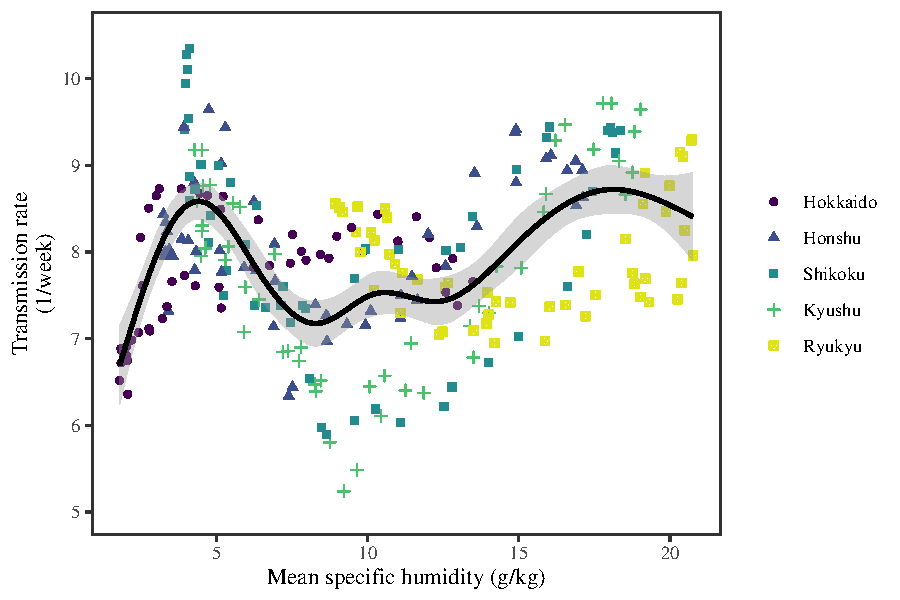
\includegraphics[width=\textwidth]{../figure/figure_joint_climate.pdf}
\caption{
\textbf{Joint relationship between the estimated periodic seasonal transmission rates and mean specific humidity across all five islands.}
Points represent the estimates across 52 weeks in each island.
The line represent a generalized additive model fit using cubic spline basis.
}
\label{fig:fig2}
\end{figure}

\pagebreak

\bibliography{perturbation}

\end{document}
